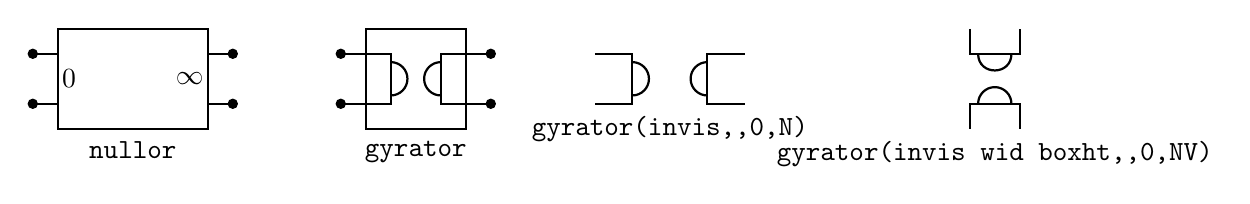
\begin{tikzpicture}[scale=2.54]
% dpic version 2020.03.01 option -g for TikZ and PGF 1.01
\ifx\dpiclw\undefined\newdimen\dpiclw\fi
\global\def\dpicdraw{\draw[line width=\dpiclw]}
\global\def\dpicstop{;}
\dpiclw=0.8bp
\dpiclw=0.8bp
\dpicdraw (0.145,-0.25) rectangle (0.895,0.25)\dpicstop
\draw (0.145,0) node[right=-2bp]{${}0$};
\draw (0.895,0) node[left=-2bp]{$\infty$};
\dpicdraw (0.145,0.125)
 --(0.02,0.125)\dpicstop
\dpicdraw[fill=black](0.02,0.125) circle (0.007874in)\dpicstop
\dpicdraw (0.145,-0.125)
 --(0.02,-0.125)\dpicstop
\dpicdraw[fill=black](0.02,-0.125) circle (0.007874in)\dpicstop
\dpicdraw (0.895,0.125)
 --(1.02,0.125)\dpicstop
\dpicdraw[fill=black](1.02,0.125) circle (0.007874in)\dpicstop
\dpicdraw (0.895,-0.125)
 --(1.02,-0.125)\dpicstop
\dpicdraw[fill=black](1.02,-0.125) circle (0.007874in)\dpicstop
\draw (0.52,-0.291511) node[below=-2bp]{\tt nullor};
\dpicdraw (1.685,-0.25) rectangle (2.185,0.25)\dpicstop
\dpicdraw (1.685,0.125)
 --(1.56,0.125)\dpicstop
\dpicdraw[fill=black](1.56,0.125) circle (0.007874in)\dpicstop
\dpicdraw (1.685,-0.125)
 --(1.56,-0.125)\dpicstop
\dpicdraw[fill=black](1.56,-0.125) circle (0.007874in)\dpicstop
\dpicdraw (2.185,0.125)
 --(2.31,0.125)\dpicstop
\dpicdraw[fill=black](2.31,0.125) circle (0.007874in)\dpicstop
\dpicdraw (2.185,-0.125)
 --(2.31,-0.125)\dpicstop
\dpicdraw[fill=black](2.31,-0.125) circle (0.007874in)\dpicstop
\dpicdraw (1.685,0.125)
 --(1.81,0.125)
 --(1.81,-0.125)
 --(1.685,-0.125)\dpicstop
\dpicdraw (1.81,-0.083333)
 ..controls (1.856024,-0.083333) and (1.893333,-0.046024)
 ..(1.893333,0)
 ..controls (1.893333,0.046024) and (1.856024,0.083333)
 ..(1.81,0.083333)\dpicstop
\dpicdraw (2.185,0.125)
 --(2.06,0.125)
 --(2.06,-0.125)
 --(2.185,-0.125)\dpicstop
\dpicdraw (2.06,0.083333)
 ..controls (2.013976,0.083333) and (1.976667,0.046024)
 ..(1.976667,0)
 ..controls (1.976667,-0.046024) and (2.013976,-0.083333)
 ..(2.06,-0.083333)\dpicstop
\draw (1.935,-0.291511) node[below=-2bp]{\tt gyrator};
\dpicdraw (2.83,0.125)
 --(3.0175,0.125)
 --(3.0175,-0.125)
 --(2.83,-0.125)\dpicstop
\dpicdraw (3.0175,-0.083333)
 ..controls (3.063524,-0.083333) and (3.100833,-0.046024)
 ..(3.100833,0)
 ..controls (3.100833,0.046024) and (3.063524,0.083333)
 ..(3.0175,0.083333)\dpicstop
\dpicdraw (3.58,0.125)
 --(3.3925,0.125)
 --(3.3925,-0.125)
 --(3.58,-0.125)\dpicstop
\dpicdraw (3.3925,0.083333)
 ..controls (3.346476,0.083333) and (3.309167,0.046024)
 ..(3.309167,0)
 ..controls (3.309167,-0.046024) and (3.346476,-0.083333)
 ..(3.3925,-0.083333)\dpicstop
\draw (3.205,-0.25) node{\tt gyrator(invis,{,}0,N)};
\dpicdraw (4.705,-0.25)
 --(4.705,-0.125)
 --(4.955,-0.125)
 --(4.955,-0.25)\dpicstop
\dpicdraw (4.913333,-0.125)
 ..controls (4.913333,-0.078976) and (4.876024,-0.041667)
 ..(4.83,-0.041667)
 ..controls (4.783976,-0.041667) and (4.746667,-0.078976)
 ..(4.746667,-0.125)\dpicstop
\dpicdraw (4.705,0.25)
 --(4.705,0.125)
 --(4.955,0.125)
 --(4.955,0.25)\dpicstop
\dpicdraw (4.746667,0.125)
 ..controls (4.746667,0.013889) and (4.913333,0.013889)
 ..(4.913333,0.125)\dpicstop
\draw (4.83,-0.291511) node[below=-2bp]{\tt gyrator(invis wid boxht,{,}0,NV)};
\end{tikzpicture}
\vspace*{-0.5\baselineskip}
